\documentclass[11pt]{article}
\usepackage[T1]{fontenc}
\usepackage{lmodern,microtype}
\usepackage[a4paper,margin=25mm]{geometry}
\usepackage{amsmath,amssymb,amsthm,mathtools,booktabs,longtable,array,graphicx,xcolor,xurl,enumitem}
\usepackage[numbers,sort&compress]{natbib}
\usepackage[colorlinks=true,linkcolor=blue!45!black,citecolor=blue!45!black,urlcolor=blue!45!black]{hyperref}
\newtheorem{theorem}{Theorem}[section]
\newtheorem{proposition}[theorem]{Proposition}
\newtheorem{lemma}[theorem]{Lemma}
\newtheorem{corollary}[theorem]{Corollary}
\theoremstyle{remark}\newtheorem{remark}[theorem]{Remark}
\newcommand{\E}{\mathbb E}
\newcommand{\PP}{\mathbb P}
\graphicspath{{../figures/}}
\hypersetup{pdftitle={Retained Moments and Discovered Neural Directions},pdfauthor={Wenyu Huang}}
\title{Retained Moments and Discovered Neural Directions\\[5pt]
\large Exact Failure Diagnostics and Online Learning Experiments}
\author{Wenyu Huang\\University of California San Diego}
\date{}

\date{Research report, September 20, 2026}
\begin{document}
\maketitle
\begin{abstract}
What information lets a learner discover useful structural changes that were
not individually specified before the data? We investigate this question by
first attempting to reduce its natural formulations to existing results.
Generic retained-moment characterization, adaptive use of a uniformly valid
coreset, and residual spectral growth fail as substantial originality claims.
We then study an exact obstruction in centered quadratic neural learning:
subtracting the current model from a stored estimate of a population moment
is different from recomputing empirical residual correlations. Without
refitting, repeated spectral births from a fixed moment are exactly one
spectral truncation. At a noiseless exact fit, the former construction almost
surely proposes a harmful unthresholded birth, whereas sample residuals
vanish. We derive its exact finite-sample variance, a fresh-residual contraction,
and a conditional width--risk bound, with complete proofs and explicit
classical dependencies. Reproducible estimator diagnostics and trained,
ordinary-start online neural comparisons distinguish supplied directions,
sample-discovered directions, refitting, retention, and fixed capacity.
Independent reviews and negative controls are retained. These results provide
an auditable research record and falsification tools; they do not establish
a substantial new general theorem of structural learning, a universally
better learner, or publication readiness.
\end{abstract}
\tableofcontents

\section{Question, evidence, and scientific status}
The motivation is information-driven adaptation of neural structure. Neither
entropy, neuron splitting, nor memory is imposed as the answer. The desired
contribution must explain a consequence not already supplied by the closest
external theorem or algorithm. This report records actual progress toward
that standard, including candidates that did not meet it.

The initial question concerned information a learner should retain to
\emph{discover} future useful operations, rather than merely validate a supplied
one. Discovery requires an optimization procedure that returns trainable
weights, and its search work and information access must be counted. A theorem
that estimates the supremum of possible gains does not necessarily return a
maximizing neuron. Conversely, when a guarantee is uniform over a fixed
function class, the eventual candidate identities may be chosen after the data
without creating an additional validity problem.

The actual starting workspace matters. It already contains finite-encoder
obstructions; a restricted activation-observation separation and high-order
splits; repeated neural growth with fresh audits; exact retained-moment
ambiguity and residual testing costs; and a 336-trajectory audit-release
study. The latter finds benefits from releasing old labels, no resolved
advantage of residual over random proposals, and stronger fixed online
controls on some tasks. None is claimed again here. The starting
1,087 non-environment files were hashed and preserved. The requested
Phase IV brief and handoff were read in full; the later actual artifacts
superseded incomplete descriptions in the handoff.

Independent investigations considered retained decision information,
noise-aware rank adaptation, coordinated high-order births, and
function-preserving changes to trainability. Three reductions explain why
several appealing central claims were rejected. The subsequent analysis
changes the scientific target to a concrete finite-sample discrepancy:
\emph{what does a stored population inverse fail to subtract when the model
has already learned part of the signal?} This has an exact answer in a
realizable quadratic neural family. Its interpretation is deliberately
bounded: the answer specializes matrix regression and stochastic
approximation. Correctness and usefulness do not establish substantial
external novelty.

\section{The novelty checkpoint and nearest results}
\label{sec:prior}
\subsection{Reductions that defeated initial candidate claims}
For unknown label means $g$ and retained linear observations $\Lambda g$, a
best-action value of the form $\sup_\theta\langle h_\theta,g\rangle$ is a
supremum of linear functionals. Foucart's nonlinear optimal-recovery
framework covers this object and bounded observation error
\cite[Theorems 1, 3; Section 2.3]{foucart}. It does not solve the neural
maximizer problem. Moving from one supplied action to a continuum therefore
does not by itself establish a new recovery theorem.

Suppose a retained objective obeys
$\sup_{f\in\mathcal F}|F(f)-\widetilde F(f)|\le\varepsilon$ on one event.
Then all adaptively chosen $f\in\mathcal F$ are covered on that event. If
$\widetilde F(\hat f)\le\inf_{f\in\mathcal F}\widetilde F(f)+\eta$, then
\[
 F(\hat f)\le\inf_{f\in\mathcal F}F(f)+2\varepsilon+\eta.
\]
This follows by inserting the two approximation inequalities around the
retained-objective optimization inequality. Strong coresets already have
this simultaneous-query meaning \cite{coresets}. The construction size,
changing encompassing class, and optimization error remain substantive;
renaming the final query a structural action does not change the argument.

Similarly, uniform score error $\varepsilon$ and optimization error $\eta$
produce a feature oracle with error $2\varepsilon+\eta$. Residual feature
search and approximate conditional-gradient oracles are existing tools
\cite[Section 2.5]{bach}. Gradient-matching retention already targets models
away from the current fit \cite{gmc}; its Appendix A.4 discusses the loss of
exact historical accumulation when embeddings change. Gradient mismatch
also already enters convergence guarantees \cite{gradmatch}. These sources
prevent claiming that a replay buffer or retained probe gradients constitute
the main contribution.

\subsection{Why quadratic neurons do not make rank learning new}
A signed quadratic network has matrix parameter
$A=\sum_j a_jw_jw_j^\top$. Thus adding a neuron is adding a symmetric rank-one
atom. GECO already chooses a leading singular direction and refits
coefficients \cite{geco}; under directional smoothness it supplies an
$O(\|A\|_*^2/k)$ approximation comparison. Restricted-curvature greedy
analysis yields stronger rates \cite[Theorem 4]{khanna}. The nonlinear
factor optimization used in our experiments is not guaranteed to perform
GECO's exact corrective minimization.

Rank-one quadratic measurements already admit stable low-rank recovery
\cite[Theorem 1]{chenchi}. Fixed overparameterized quadratic networks also
learn directions \cite[Theorem 1.2]{lima}, and incremental-rank trajectories
of gradient descent are established under matrix-sensing assumptions
\cite[Theorem 4.1]{jin}. Raw Gaussian outer-product sensing does not satisfy
ordinary Frobenius $\ell_2/\ell_2$ RIP merely because the covariates are
Gaussian. This blocks an otherwise tempting incorrect transfer.

The residual matrix update analyzed below is stochastic gradient descent in
matrix coordinates. With rank projection it has the stochastic iterative
hard-thresholding form \cite[Algorithm 1, Theorem 1]{stoiht}. Our exact
Gaussian moment calculation directly handles fresh unbounded Gaussian
batches, but does not supply a novel optimization principle. Signal-induced
failure of untrimmed spectral initialization also has explicit prior
analysis \cite[Section 2.2]{twf}. Empirical residual cross-moments and
spectral neural additions have a close structural-learning precedent
\cite[Propositions 3.2--3.3]{tiny}.

\subsection{A theorem-level comparison summary}
\begin{longtable}{>{\raggedright\arraybackslash}p{.14\linewidth}>{\raggedright\arraybackslash}p{.30\linewidth}>{\raggedright\arraybackslash}p{.45\linewidth}}
\toprule
Claim & Closest result / mapping & Disposition and missing step\\\midrule
\endhead
Best future gain from moments & Sup-linear optimal recovery \cite{foucart} &
Inherited value recovery; finding a trainable maximizer within a resource
budget is additional.\\
Adaptive retained objective & Strong coresets \cite{coresets} &
Uniformity already covers data-dependent identities in its fixed class;
changing-class online construction is not supplied.\\
Residual neuron discovery & Convex neural oracle and GECO \cite{bach,geco} &
Rank-one atom search is known; no new direction-search theorem here.\\
Fixed-summary birth path & Spectral decomposition & Exact diagnostic;
with no refit the path equals a single hard truncation.\\
Fresh residual correction & Stochastic gradient / StoIHT \cite{stoiht} &
Exact Gaussian constants and a noise-free false-growth witness are proved;
$O(d^2)$ batch bound is not an optimal low-rank rate.\\
Selected width certificate & Hard threshold / penalized rank &
Conditional perturbation and oracle inequality; the stated finite-sample
radius is conservative and requires norm bounds.\\
Actual trained histories & Present saved runs & Empirical evidence specific
to observed-data proposals, optimizer, tasks and accounting; no theorem of
universal structural superiority.\\\bottomrule
\end{longtable}

The full \texttt{NOVELTY\_MATRIX.md} identifies source versions, observation
interfaces, resources, guarantees, attempted reductions, and unresolved
risks. The current representation-certification source was checked at v2,
not inherited as v1 \cite{huang}; its repair discussion is outside the fixed
kernel result. A source-level counterexample warning about a different
current spectral claim is included in Appendix~\ref{app:source}; we do not
use that claim as a black-box theorem.

% Self-contained body; main.tex supplies amsmath, amssymb, amsthm and
% theorem/proposition/corollary/remark environments. No bespoke macros.
\section{An exact quadratic diagnostic and its limits}
\label{sec:quadratic-theory}

The results in this section are specializations of classical Gaussian
moment identities, spectral approximation, and stochastic approximation.
Their purpose is to distinguish population inversion, finite-sample
estimation, and actual empirical optimization. They do not establish a
substantially original learning algorithm or an advantage of autonomous
neural growth. All probability and expectation statements below are exact
under the stated model; the numerical checks in the experiments are
separate evidence.

Fix integers $d,n\geq1$. Matrices are real and symmetric unless indicated
otherwise, with inner product $\langle A,B\rangle=\operatorname{tr}(AB)$.
Write $\|\cdot\|_F$, $\|\cdot\|_{\mathrm{op}}$, and $\|\cdot\|_*$ for
Frobenius, operator, and nuclear norms. Set
\[
 X\sim N(0,I_d),\qquad H(X)=XX^\top-I_d,\qquad
 q_A(X)=\langle A,H(X)\rangle.
\]
The unknown fixed teacher is $A_*$. Labels obey
\begin{equation}
 Y=q_{A_*}(X)+\xi,\qquad
 \mathbb E\xi=0,\quad \mathbb E\xi^2=\sigma^2<\infty,
 \quad \xi\ \hbox{independent of }X.
 \label{eq:quadratic-model}
\end{equation}
Distinct examples have independent copies of $(X,\xi)$. Define population
squared risk $R(B)=\mathbb E[(Y-q_B(X))^2]$.

A signed centered quadratic network
\[
 f(x)=\sum_{j=1}^k a_j\{(w_j^\top x)^2-\|w_j\|_2^2\}
\]
represents $B=\sum_{j=1}^k a_jw_jw_j^\top$. Its minimum width is
$\operatorname{rank}(B)$: any such sum has rank at most $k$, while an
eigendecomposition represents $B$ with exactly its number of nonzero
eigenvalues. The zero predictor has width zero. A constant output can
implement the centering. Negative $a_j$ are allowed throughout; restricting
all outputs to be nonnegative changes the operation class to positive
semidefinite matrices and does not preserve every result below.

\subsection{Population geometry}

\begin{theorem}[T1: Gaussian quadratic geometry]
\label{thm:quadratic-geometry}
For symmetric $A,B$,
\begin{equation}
 \mathbb E[q_A(X)q_B(X)]=2\operatorname{tr}(AB).
 \label{eq:quadratic-isometry}
\end{equation}
Consequently, under \eqref{eq:quadratic-model},
\begin{equation}
 R(B)-R(A_*)=2\|B-A_*\|_F^2,
 \qquad \frac12\mathbb E[YH(X)]=A_*.
 \label{eq:quadratic-risk-moment}
\end{equation}
\end{theorem}
\begin{proof}
For standard Gaussian coordinates, second and fourth moments are
\[
 \mathbb E[X_iX_j]=\delta_{ij},\qquad
 \mathbb E[X_iX_jX_kX_l]
 =\delta_{ij}\delta_{kl}+\delta_{ik}\delta_{jl}
  +\delta_{il}\delta_{jk}.
\]
Subtracting the product of second moments yields
$\mathbb E[H_{ij}H_{kl}]=\delta_{ik}\delta_{jl}
+\delta_{il}\delta_{jk}$. Multiply by $A_{ij}B_{kl}$ and sum all indices.
The symmetry of $A,B$ gives \eqref{eq:quadratic-isometry}. Taking one
matrix to be an arbitrary symmetric test matrix gives
$\mathbb E[q_A(X)H(X)]=2A$.

Let $E=A_*-B$. Independence and zero mean of $\xi$ give
$\mathbb E[\xi q_E(X)]=0$ and $\mathbb E[\xi H(X)]=0$.
Thus $R(B)=\mathbb E[q_E(X)^2]+\sigma^2
=2\|E\|_F^2+\sigma^2$, while $R(A_*)=\sigma^2$.
The second identity follows by taking the moment of $Y$.
\end{proof}

Without centering, the corresponding quadratic prediction difference has
second moment $2\|A-B\|_F^2+\operatorname{tr}(A-B)^2$.
Thus centering is part of the model, not an inconsequential convention.

\subsection{What repeated growth from a fixed summary computes}

\begin{theorem}[T2: fixed-summary spectral growth]
\label{thm:spectral-collapse}
Fix a symmetric matrix $S$ and set $B_0=0$. At each nonterminal step,
select a unit eigenvector $v_t$ of $S-B_t$ whose eigenvalue $\lambda_t$
has maximum absolute value, and set
\[
 B_{t+1}=B_t+\lambda_tv_tv_t^\top.
\]
For a fixed $\tau\geq0$, terminate before this update if
$|\lambda_t|\leq\tau$. Every nonzero update selects a previously
unselected eigencomponent of $S$, in nonincreasing absolute-eigenvalue
order. In at most $d$ updates the terminal result is
\begin{equation}
 B_{\rm stop}=\sum_{j:\,|s_j|>\tau}s_ju_ju_j^\top,
 \qquad S=\sum_{j=1}^d s_ju_ju_j^\top.
 \label{eq:hard-truncation}
\end{equation}
Intermediate truncations can be nonunique at ties.
The final strict-threshold result is invariant to these choices.
\end{theorem}
\begin{proof}
We maintain an orthonormal set of selected eigenvectors of $S$ such that
$B_t$ is the sum of their original eigencomponents. This holds at $t=0$.
The residual $S-B_t$ is zero on their span and equals $S$ on its
orthogonal complement. If a nonzero residual eigenvalue remains, every
unit eigenvector with that nonzero eigenvalue is orthogonal to the
selected span. It is an eigenvector of $S$ with the same eigenvalue.
The update therefore extends the orthonormal selected set and removes
exactly that one component from the residual. Selecting maximum absolute
value establishes the order. At most $d$ nonzero components can be
removed. The stopping rule removes all and only components with
absolute eigenvalue strictly greater than $\tau$, proving
\eqref{eq:hard-truncation}.

Within an eigenspace with the same signed eigenvalue, any orthonormal
basis is permissible. If $s$ and $-s$ are tied in absolute value, one
may choose either eigenspace, but arbitrary mixtures across them need
not be eigenvectors and are not allowed by the algorithm. When the
residual is zero, the rule terminates, including when $\tau=0$.
\end{proof}

The directions in this construction can be learned from labels through
$S$. Nevertheless, after $S$ has been formed the trajectory is precisely
an eigendecomposition procedure. A one-shot estimator with the same
$S$, threshold and eigensolver produces the same predictor. This statement
does not identify the trajectory of a method that subsequently refits
neurons using empirical loss.

For an observed dataset, define
\begin{equation}
 S_n=\frac1{2n}\sum_{i=1}^nY_iH_i,
 \qquad
 T_n(B)=\frac1{2n}\sum_{i=1}^n\langle B,H_i\rangle H_i,
 \quad H_i=H(X_i).
 \label{eq:empirical-moment-operator}
\end{equation}
The actual residual moment satisfies the algebraic identity
\begin{equation}
 G_n(B):=\frac1{2n}\sum_{i=1}^n
       \{Y_i-q_B(X_i)\}H_i=S_n-T_n(B).
 \label{eq:actual-residual}
\end{equation}
It is the negative Euclidean matrix gradient of
$L_n(B)=(4n)^{-1}\sum_i\{Y_i-q_B(X_i)\}^2$.
The surrogate $S_n-B$ replaces the empirical operator $T_n$ by its
population mean. For fixed $B$ independent of the sample,
$\mathbb E[T_n(B)\mid B]=B$; equality on the realized sample does not
follow. If $B$ uses the same sample, even this conditional identity can
fail.

\begin{remark}[An explicit adaptive-reuse counterexample]
\label{rem:adaptive-counterexample}
Take $d=n=1$, $A_*=1$, $\sigma=0$, and $H=X^2-1$. Then $Y=H$.
Choose $B=S_1=H^2/2$, which is a legitimate data-dependent estimate.
Equation~\eqref{eq:empirical-moment-operator} gives $T_1(B)=B^2$.
Thus $\mathbb E[T_1(B)\mid B]=B^2$, generally different from $B$.
A same-sample residual correction is $C=B+G_1(B)=2B-B^2$, so
$|C-1|^2=(B-1)^4$. The fresh-block conditional variance in the next
theorem would instead be $14(B-1)^2$ and does not apply here.
\end{remark}

For exact empirical residual evaluation at arbitrary $B$, one must apply
$T_n$, using replay, its stored operator, or an equivalent representation.
In orthonormal symmetric coordinates, $T_n$ is one half the empirical
Gram operator of the $d(d+1)/2$ centered quadratic features. Its entries
include fourth-order input moments. This is the ordinary regression
normal equation; it is not a lower bound on physical memory, and no
minimum-bit claim follows from it.

\subsection{Exact sampling variance and fresh corrections}

\begin{theorem}[T3: variance of a fresh residual correction]
\label{thm:residual-variance}
Define
\[
 c_d=\frac{d^2+9d+14}{2}.
\]
For any fixed symmetric $E$ and $Z_E=\tfrac12q_E(X)H(X)$,
\begin{equation}
 \mathbb E Z_E=E,\qquad
 \mathbb E\|Z_E-E\|_F^2
 =c_d\|E\|_F^2+2\operatorname{tr}(E)^2.
 \label{eq:exact-design-variance}
\end{equation}
Let $\mathcal F$ contain the complete history before a new block, and
let $B$ be a square-integrable symmetric $\mathcal F$-measurable matrix.
Conditional
on $\mathcal F$, the new $n$ observations are independent copies of
\eqref{eq:quadratic-model} and independent of $\mathcal F$. Set
\[
 E=A_*-B,\qquad
 C=B+\frac1{2n}\sum_{i=1}^n
             \{Y_i-q_B(X_i)\}H_i.
\]
Then
\begin{align}
 \mathbb E[C\mid\mathcal F]&=A_*,\\
 \mathbb E[\|C-A_*\|_F^2\mid\mathcal F]
 &=\frac{c_d\|E\|_F^2+2\operatorname{tr}(E)^2
                +\sigma^2d(d+1)/4}{n}.
 \label{eq:fresh-conditional-variance}
\end{align}
\end{theorem}
\begin{proof}
Write $s=\|X\|_2^2$ and $U=X/\|X\|_2$, with any definition at
$X=0$, a null event. The radius $s\sim\chi_d^2$ is independent of the
uniform direction $U$ on the unit sphere. Put
$\theta=\operatorname{tr}(E)$ and $v=\|E\|_F^2$.
Rotational symmetry, or the Gaussian fourth-moment identity applied
before dividing out the radius, gives
\[
 \mathbb E[U^\top EU]=\frac{\theta}{d},\qquad
 \mathbb E[(U^\top EU)^2]=\frac{\theta^2+2v}{d(d+2)}.
\]
Indeed, the second formula follows from
$\mathbb E[(X^\top EX)^2]=\theta^2+2v$ and
$\mathbb E[s^2]=d(d+2)$ by radial independence.
Since $q_E=sU^\top EU-\theta$,
\begin{equation}
 \mathbb E[q_E^2\mid s]
 =\frac{(\theta^2+2v)s^2}{d(d+2)}
       -\frac{2\theta^2s}{d}+\theta^2.
 \label{eq:conditional-radial-moment}
\end{equation}
The chi-square moments are
\[
 \mathbb E[s^j]=\prod_{l=0}^{j-1}(d+2l),\qquad j=1,2,3,4.
\]
Substitute these into \eqref{eq:conditional-radial-moment}, after
multiplying respectively by $1,s,s^2$, to obtain
\begin{align*}
 \mathbb E[q_E^2]&=2v,\\
 \mathbb E[q_E^2s]&=2(d+4)v,\\
 \mathbb E[q_E^2s^2]&=8\theta^2+2(d+4)(d+6)v.
\end{align*}
Also $\|H\|_F^2=s^2-2s+d$. Hence
\begin{align*}
 \mathbb E[q_E^2\|H\|_F^2]
 &=8\theta^2+2\{(d+4)(d+6)-2(d+4)+d\}v\\
 &=8\theta^2+2(d^2+9d+16)v.
\end{align*}
By Theorem~\ref{thm:quadratic-geometry}, $\mathbb E Z_E=E$.
The identity
$\mathbb E\|Z_E-E\|_F^2=\mathbb E\|Z_E\|_F^2-\|E\|_F^2$
now proves \eqref{eq:exact-design-variance}.

For the noisy single-example correction, let
$W=Z_E+\tfrac12\xi H$. Conditional on the past, $E$ is fixed.
Independence and zero mean of $\xi$ eliminate all cross terms between
$Z_E-E$ and $\xi H$. Furthermore,
\[
 \mathbb E\|H\|_F^2=d(d+2)-2d+d=d(d+1).
\]
Consequently $\mathbb E[W\mid\mathcal F]=E$ and
\[
 \mathbb E[\|W-E\|_F^2\mid\mathcal F]
 =c_d\|E\|_F^2+2\theta^2+\frac{\sigma^2d(d+1)}4.
\]
The $n$ conditionally independent centered matrices $W_i-E$ have zero
expected pairwise Frobenius inner products. Their average therefore
has exactly $1/n$ times this variance. Since
$C-A_*=n^{-1}\sum_i(W_i-E)$, both claims follow.
\end{proof}

\begin{corollary}[Contraction with genuinely fresh blocks]
\label{cor:fresh-contraction}
Initialize a deterministic finite $B_0$ and repeat the unprojected update
in Theorem~\ref{thm:residual-variance}, with block size $n$ and fresh
independent blocks. Set
\[
 \kappa=\frac{c_d+2d}{n},\qquad
 \nu=\frac{\sigma^2d(d+1)}{4n}.
\]
For all integers $T\geq0$,
\begin{equation}
 \mathbb E\|B_T-A_*\|_F^2
 \leq\kappa^T\|B_0-A_*\|_F^2
       +\nu\sum_{j=0}^{T-1}\kappa^j.
 \label{eq:contraction-sum}
\end{equation}
If $n>c_d+2d$, the sum equals
$(1-\kappa^T)/(1-\kappa)$ and $\kappa<1$.
If instead every update is replaced by a best symmetric rank-at-most-$r$
Frobenius approximation, with known $r\geq\operatorname{rank}(A_*)$,
the same statement holds with $\kappa$ replaced by $4\kappa$ and $\nu$
by $4\nu$. That sufficient contraction condition is
$n>4(c_d+2d)$.
\end{corollary}
\begin{proof}
Cauchy--Schwarz on the eigenvalues gives
$\operatorname{tr}(E)^2\leq d\|E\|_F^2$.
Apply this inequality in \eqref{eq:fresh-conditional-variance}, then
take expectations. The resulting recurrence is
$e_{t+1}\leq\kappa e_t+\nu$, where
$e_t=\mathbb E\|B_t-A_*\|_F^2$. The right side is finite by induction;
iterating the recurrence proves \eqref{eq:contraction-sum}.
For rank truncation, the feasibility of $A_*$ and best-approximation
property give
\[
 \|P_r(C)-A_*\|_F
 \leq\|P_r(C)-C\|_F+\|C-A_*\|_F
 \leq2\|C-A_*\|_F.
\]
Square and condition on the past to obtain the stated factors of four.
A fixed measurable tie convention suffices to define the projection.
\end{proof}

This result has an $O(d^2)$ sufficient block size and an unconstrained
output that can require $d$ signed neurons. A supplied rank is privileged
information. These facts do not establish an optimal $O(dr)$ sample
bound, selected width, or a computational advantage over fixed-width
training. The matrix update is stochastic gradient descent for the
matrix-coordinate loss in \eqref{eq:actual-residual}; it is not the same
update as gradient descent in neuron factors. The exact variance formula
also quantifies the familiar control-variate effect of subtracting a
previously fitted predictor before estimating a residual.

\subsection{A wrong surrogate can propose harmful growth at an exact fit}

\begin{theorem}[T4: false growth at the optimum]
\label{thm:false-growth}
Assume $\sigma=0$ and $A_*\ne0$. From any $n\geq1$ fresh observations
form $S_n$ in \eqref{eq:empirical-moment-operator}, and consider the exact
fit $B=A_*$. Put $D=S_n-A_*$ and let $(\lambda,v)$ be a top-absolute-value
unit eigenpair of $D$. Consider the signed neuron update
$B'=A_*+\lambda vv^\top$. Its true risk increase and its improvement in
the surrogate $\widetilde R_{S_n}(B)=2\|B-S_n\|_F^2$ coincide:
\begin{equation}
 R(B')-R(A_*)
 =\widetilde R_{S_n}(A_*)-\widetilde R_{S_n}(B')
 =2\lambda^2.
 \label{eq:false-growth-gain}
\end{equation}
This quantity is strictly positive almost surely. With
$V=c_d\|A_*\|_F^2+2\operatorname{tr}(A_*)^2$,
\begin{equation}
 \frac{2V}{dn}
 \leq\mathbb E[R(B')-R(A_*)]
 \leq\frac{2V}{n}.
 \label{eq:false-growth-expectation}
\end{equation}
In contrast, the actual empirical residual moment at $A_*$ is exactly
zero on every sample.
\end{theorem}
\begin{proof}
Since $Y_i=q_{A_*}(X_i)$, every actual residual at $A_*$ is zero, proving
the last assertion. The population risk identity and
$\|vv^\top\|_F=1$ yield $R(B')-R(A_*)=2\lambda^2$.
Also $\langle D,vv^\top\rangle=v^\top Dv=\lambda$, so
\[
 \|D-\lambda vv^\top\|_F^2
 =\|D\|_F^2-2\lambda^2+\lambda^2
 =\|D\|_F^2-\lambda^2.
\]
This proves the surrogate identity.

Apply Theorem~\ref{thm:residual-variance} with $B=0$ and $\sigma=0$
to obtain $\mathbb E\|D\|_F^2=V/n>0$. At least one entry of $D$
therefore has positive second moment. Every entry is a polynomial in
the $nd$ independent Gaussian coordinates. At least one is a nonzero
polynomial; its zero set has Lebesgue measure zero. For completeness,
this property follows by induction on the number of variables: view a
nonzero multivariate polynomial as a polynomial in its last variable;
outside the common zero set of its nonzero coefficient polynomials,
it has finitely many roots, and Fubini's theorem finishes the induction.
The joint Gaussian law has a density, so $\mathbb P(D=0)=0$.
Thus $|\lambda|=\|D\|_{\mathrm{op}}>0$ almost surely.
Finally,
$\|D\|_F^2/d\leq\|D\|_{\mathrm{op}}^2\leq\|D\|_F^2$;
expectations give \eqref{eq:false-growth-expectation}.
\end{proof}

The exact fit is an oracle diagnostic checkpoint, not a checkpoint claimed
to be learned by the experimental controller. The theorem concerns the
unrestricted positive-score surrogate rule, with signed additions and
without a nonzero uncertainty threshold. It does not assert that a
thresholded or independently audited rule must accept. Any such accepted
nonzero update at the exact fit is harmful, but its acceptance probability
and expected accepted loss require a separate analysis. The theorem is
not a lower bound for every algorithm using $S_n$.

\subsection{A conditional width and risk certificate}

\begin{theorem}[Hard-threshold oracle inequality]
\label{thm:threshold-oracle}
Let $A_*,S$ be arbitrary symmetric matrices and let $b\geq0$ satisfy
$\|S-A_*\|_{\mathrm{op}}\leq b$. Let $s_1(A_*)\geq\cdots\geq s_d(A_*)$
denote the singular values of $A_*$, and let $\widehat A$ retain exactly
the eigencomponents of $S$ with absolute eigenvalue strictly greater
than $2b$. Then
\begin{align}
 \operatorname{rank}(\widehat A)
 &\leq\#\{j:s_j(A_*)>b\},
 \label{eq:threshold-rank}\\
 \|\widehat A-A_*\|_F^2
 &\leq\min_{0\leq r\leq d}
 \left\{3\sum_{j>r}s_j(A_*)^2+16b^2r\right\}.
 \label{eq:threshold-risk}
\end{align}
The corresponding excess prediction risk under
\eqref{eq:quadratic-model} is twice the bound in
\eqref{eq:threshold-risk}.
\end{theorem}
\begin{proof}
The singular-value perturbation bound
$|s_j(S)-s_j(A_*)|\leq\|S-A_*\|_{\mathrm{op}}$ implies that
$s_j(S)>2b$ entails $s_j(A_*)>b$, proving
\eqref{eq:threshold-rank}. One way to see this perturbation bound is to
apply the variational characterization
$s_j(M)=\min_{\dim W=d-j+1}\max_{u\in W,\|u\|=1}\|Mu\|$
and the triangle inequality, then interchange $S$ and $A_*$.

Hard thresholding at $2b$ minimizes, over symmetric $B$,
\[
 \|S-B\|_F^2+4b^2\operatorname{rank}(B).
\]
To justify this without a separate approximation theorem, let $B$ have
rank at most $r$ and let $P$ be the orthogonal projector onto its column
space. Then
\[
 \|S-B\|_F^2\geq\|(I-P)S\|_F^2
 =\operatorname{tr}(S^2)-\operatorname{tr}(PS^2).
\]
In an eigenbasis of $S^2$ ordered by decreasing eigenvalue, write
$p_j=u_j^\top Pu_j$. Since $0\leq p_j\leq1$ and
$\sum_jp_j=\operatorname{rank}(P)\leq r$,
$\operatorname{tr}(PS^2)\leq\sum_{j=1}^r s_j(S)^2$.
Retaining the largest $r$ singular components attains this bound and is
realizable as a symmetric eigencomponent sum. For each component,
retaining its value costs $4b^2$, whereas omitting it costs its squared
eigenvalue. At equality both choices minimize the objective, and the
theorem specifies omission.

Fix $r\in\{0,\ldots,d\}$ and let $A_{*,r}$ be a best symmetric
rank-at-most-$r$ approximation to $A_*$. Put
$k=\operatorname{rank}(\widehat A)$,
$e=\|\widehat A-A_*\|_F$, and
$a=\|A_{*,r}-A_*\|_F$. Comparing penalized objectives and expanding
around $A_*$ gives
\[
 e^2\leq a^2+2\langle S-A_*,\widehat A-A_{*,r}\rangle
                  +4b^2(r-k).
\]
The use of $r$ rather than the possibly smaller rank of $A_{*,r}$ can
only enlarge the right side. Operator/nuclear duality, the inequality
$\|M\|_*\leq\sqrt{\operatorname{rank}(M)}\|M\|_F$, and the triangle
inequality imply
\[
 e^2\leq a^2+2b\sqrt{k+r}(e+a)+4b^2(r-k).
\]
Apply $2b\sqrt{k+r}e\leq e^2/2+2b^2(k+r)$ and
$2b\sqrt{k+r}a\leq a^2/2+2b^2(k+r)$. Rearranging yields
$e^2\leq3a^2+16b^2r$. Finally,
$a^2=\sum_{j>r}s_j(A_*)^2$, and $r$ was arbitrary.
The prediction statement follows from
Theorem~\ref{thm:quadratic-geometry}. These arguments also cover $b=0$;
in that case $S=A_*$ and $\widehat A=A_*$ directly.
\end{proof}

The strict inequality in the threshold is necessary for the stated
width bound: for $d=1$, $b=1$, $A_*=1$, and $S=2$, retaining the component
at equality gives rank one, while the right side of
\eqref{eq:threshold-rank} is zero. The risk bound alone allows either
choice at equality because both minimize the penalized objective.

An explicit, conservative finite-sample radius follows without assuming
an optimal concentration theorem. For the raw moment $S_n$, let
\[
 V_* = c_d\|A_*\|_F^2+2\operatorname{tr}(A_*)^2
                +\frac{\sigma^2d(d+1)}4.
\]
Theorem~\ref{thm:residual-variance} gives
$\mathbb E\|S_n-A_*\|_F^2=V_*/n$. For any deterministic known
$\overline V\geq V_*$ and $\delta\in(0,1)$, take
$b=\sqrt{\overline V/(n\delta)}$. Markov's inequality and
$\|M\|_{\mathrm{op}}\leq\|M\|_F$ show that the assumptions of
Theorem~\ref{thm:threshold-oracle} hold with probability at least
$1-\delta$. If $\overline V=0$, the moment is exact almost surely.
Unknown teacher norms cannot simply be substituted by same-sample point
estimates without additional uncertainty control. This radius is
conservative and signal dependent; it does not establish the optimal
noisy low-rank rate. The oracle inequality is standard hard-threshold
reasoning and is included to make that limitation explicit.

\section{Reproducible diagnostics of the exact mechanism}
\label{sec:moment-experiments}
The estimator study was specified in
\texttt{research/MOMENT\_DIAGNOSTIC\_PROTOCOL.md} before execution. It has
64 paired independent seeds, two noise levels, dimension eight, and eight
fresh batches of 512 observations. For each seed the unknown teacher is a
random rotation of $\operatorname{diag}(1,.3,0,\ldots,0)$. The four
estimators see the same chronological observations: pooled raw moment;
fresh-residual full-matrix correction; rank-two-truncated correction; and
lifted least squares. The rank-two arm is explicitly privileged by knowing
the teacher rank. Lifted least squares retains the normal-equation Gram and
right-hand side in 36-dimensional symmetric coordinates. It is a competent
larger-state control, not an equal-storage comparator.

The raw archive contains all 128 input/label arrays and every stage's four
matrix estimates, yielding 1,024 stage records. An independent reconstruction
recomputed all four estimators, risks, moment expectations and false-birth
increases; maximum estimate discrepancy was $1.78\times10^{-15}$ and
maximum risk discrepancy $3.56\times10^{-15}$. Separate five-point tensor
Gauss--Hermite integration verifies the polynomial identities for 20 matrices
in dimensions one through four. At five nodes per coordinate it integrates
these degree-eight polynomials exactly in ideal arithmetic; floating-point
agreement is a check rather than the proof. Tied signs, all-zero spectra,
strict-threshold equality and the invalid same-block conditioning example
were also checked.

\begin{table}[t]
\centering\small
\begin{tabular}{lrr}
\toprule
Estimator & Noise SD $0$ & Noise SD $.1$\\\midrule
Pooled raw moment & $0.037405$ & $0.037583$\\
Fresh residual correction & $4.33\times10^{-7}$ & $0.000826$\\
Known-rank correction & $8.73\times10^{-9}$ & $0.000306$\\
Lifted least squares & $2.73\times10^{-31}$ & $0.000092$\\
\bottomrule
\end{tabular}

\caption{Mean excess squared prediction risk after 4,096 labels over 64
independent seeds. These are estimator diagnostics, not trained-factor
neural trajectories. Full intervals and raw outcomes are in
\texttt{results/moments/findings.json}. The last two rows have explicitly
different prior information or retained-state requirements.}
\label{tab:moments}
\end{table}

The noiseless fresh correction removes much of the raw estimator's
signal-induced error. This supports the mechanism, but not a novel
statistical advantage: ordinary lifted least squares solves this small
well-specified regression essentially to machine precision. Under noise it
also has lower risk. Beating the raw moment alone therefore would be a weak
algorithmic comparison.

At the exact noiseless teacher, every tested stale-summary birth increases
true risk; the smallest recorded increase is $.004771$. This evaluates the
oracle checkpoint in the negative theorem, not an implemented learner
secretly receiving the teacher. Its purpose is to falsify the claim that
$S_n-B$ equals finite-sample residual correlation. A valid uncertainty gate
could reject these proposals. Safe rejection, however, would not prove that
a useful next feature had been discovered.

The exact expected final raw risk is $.041567$ without label noise, whereas
the 64-run mean is $.037405$ with descriptive $t$ interval
$[.034092,.040718]$. The expectation lies outside this particular interval.
We preserve that discrepancy: the statistic has a heavy-tailed polynomial
Gaussian distribution, and a nominal finite-replicate $t$ interval is not an
exact confidence procedure for its mean. Independent exact quadrature and
raw reconstruction support the identity; simulations neither replace its
proof nor guarantee nominal interval coverage. The analogous noisy mean
uses paired inputs and is not an independent replication of this
fluctuation. No additional seeds were selected to improve the agreement.

The conditional width theorem is also not automatically a useful
finite-sample selector. Here $V=85.13$ without noise. At $n=4096$ and
$\delta=.05$, the crude valid radius is $b=\sqrt{V/(n\delta)}\approx.645$;
its threshold $2b$ exceeds the largest teacher eigenvalue one. A conservative
bound can reject nearly all growth despite an easy learnable problem. This
separates an existence/validity calculation from useful selection power.

\begin{figure}[t]
\centering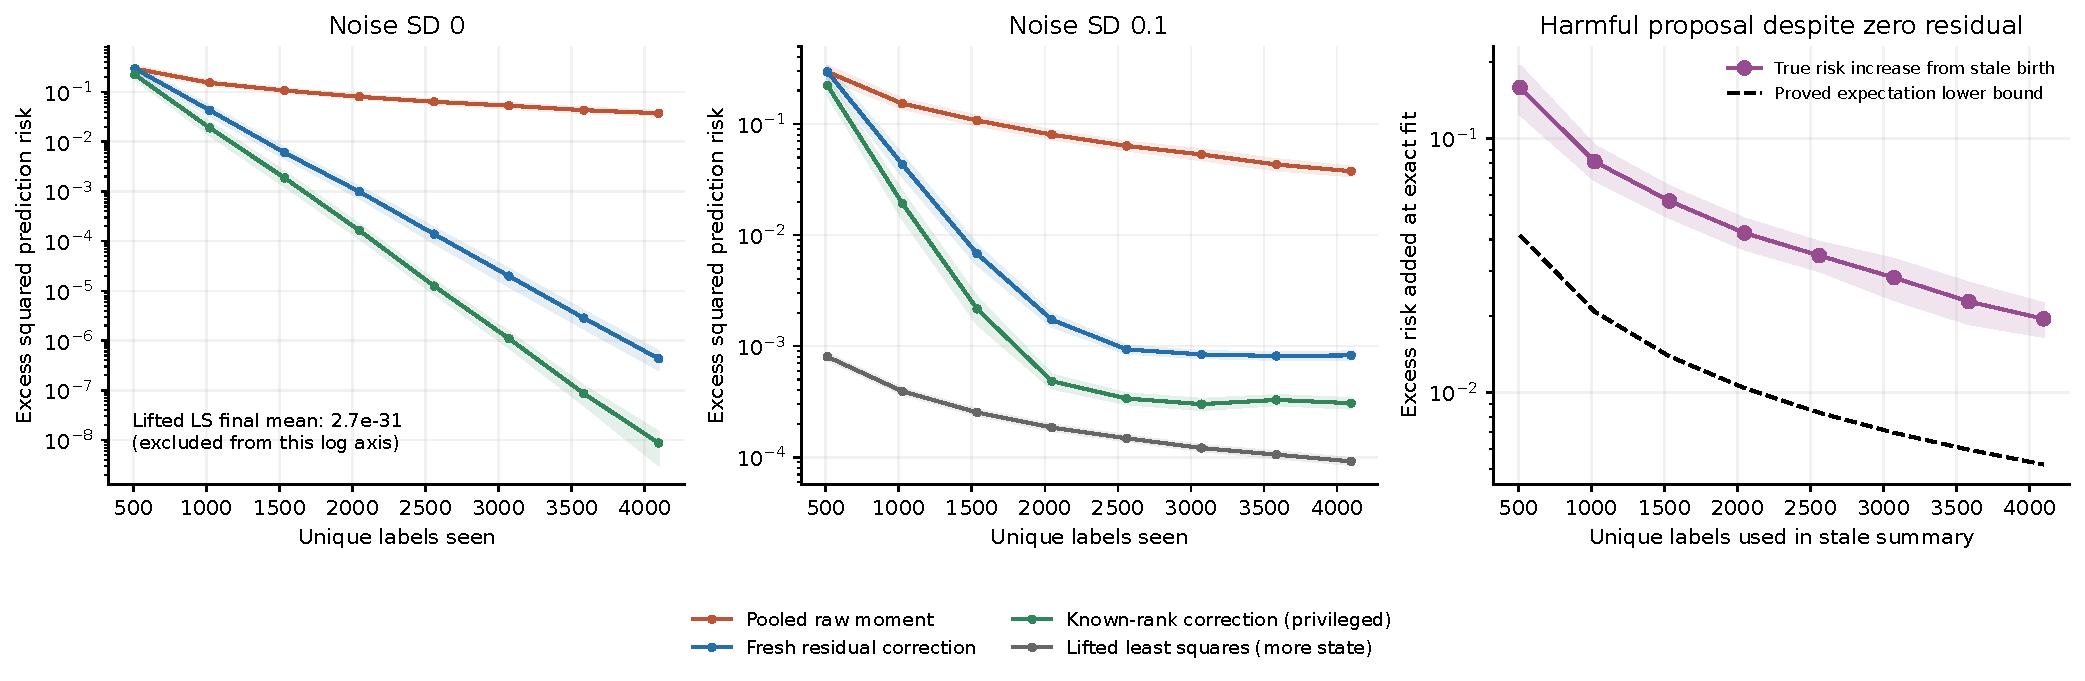
\includegraphics[width=\linewidth]{moment_diagnostics.pdf}
\caption{Saved estimator diagnostics. Shading is a descriptive 95\%
$t$ interval across 64 runs. Left and center compare chronological estimators;
the essentially zero noiseless lifted-LS endpoint is annotated instead of
stretching the log axis. Right evaluates the \emph{privileged exact-fit}
checkpoint and compares the harmful stale-birth increase with its proved
expectation lower bound. It is not a trained-method trajectory.}
\end{figure}

The simulator retains the entire generated archive for auditing, including
all arms and teacher matrices. Named array sizes are not total persistent
or peak memory measurements. An independent reviewer caught an ambiguous
metadata field; the originally executed source and metadata are preserved,
and \texttt{ACCOUNTING\_CORRECTION.md} states the correction. The numerical
code and outputs did not change. No memory superiority is inferred from
this diagnostic. The separate neural studies count learner arrays and
sample accesses under their own explicit interfaces.

\section{A controlled learner with discovered quadratic directions}
\label{sec:experiments}

We next ask whether the distinction between raw target moments and residual
moments improves an actual trained learner. This study implements the
mechanisms as conventional ingredients; it is not a new spectral algorithm.
No candidate receives a teacher direction. The principal negative result is
that a better initial direction need not retain its advantage after fully
trainable refitting, and an apparent final-risk benefit is sensitive to a
simple replay control.

\subsection{Frozen populations, data access and optimization}
All inputs have distribution $N(0,I_{12})$. Two quadratic conditional means
are $q_A(x)=x^\top A x-\operatorname{tr}(A)$, with nonzero eigenvalues
$(.8,.45)$ and $(.65,-.5,.3,-.2)$, respectively. The first has no observation
noise; the second has independent Gaussian noise with standard deviation
$.3$. A null task has mean zero and noise standard deviation $.5$.
The nonlinear task uses a hidden orthogonal rotation $z=U^\top x$ and mean
$.8\tanh(1.5z_1)\tanh(1.5z_2)+.4\sin z_3$, with noise standard deviation
$.2$. Task rotations are fixed independently of run seeds and hidden from
all learners. All labels, teacher parameters and evaluator inputs are saved.

The learned model is
\[
 f_{W,a,c}(x)=c+\sum_{j=1}^k a_j\{(w_j^\top x)^2-\|w_j\|^2\}.
\]
Every hidden vector, output coefficient and intercept trains. Initial
vectors are normalized Gaussian draws and initial coefficients have standard
deviation $.01$. Seven arrivals each reveal 1,024 labels. The current block
and an old reservoir form the fitting pool; the block enters the reservoir
only after fitting. Thus all 7,168 labels arrive at the same times, with no
future data granted to the fixed comparator. Growing arms start at width
one and receive six scheduled additions, ending at seven. This design isolates
discovered directions; it does not claim autonomous width selection or safe
rejection. New coefficients start at zero, preserving the current prediction
before ordinary, potentially risk-increasing training.

Seven arms compare: historical-moment eigenbirth, old-reservoir residual
 eigenbirth, fresh-block residual eigenbirth, four learned residual probes,
random growth with reservoirs of 128 and 138 examples, and a fixed width-seven
online learner with 138-example replay. The historical arm stores 128 examples
and $S_n=n^{-1}\sum_i y_i(x_ix_i^\top-I)/2$, and selects the eigenvector of
largest absolute eigenvalue of $S_n-B$, where $B=\sum_j a_jw_jw_j^\top$.
Residual eigenbirth instead forms
$\{\overline{(y-f)x x^\top}-\overline{(y-f)}I\}/2$ on its permitted
old reservoir or current block. It therefore includes the current intercept
term. The zero-intercept theoretical variance formulas are not claimed as
exact variance identities for every fitted checkpoint.

Learned probes maximize squared empirical residual covariance divided by
candidate second moment plus $.001$, with twenty steps and four random
starts. This is an established residual-feature objective. Directions are
selected from observations and then all network parameters are refitted.
Random additions use the same type of ordinary initial direction. The fixed
learner knows the prescribed capacity cap, not the teacher rank.

Each arrival permits two million arithmetic-proxy units, including moment
accumulation, candidate passes, eigendecomposition and fitting. Saved search
work becomes additional training. Full-gradient work is charged at
$3dk+4k+3$ per example; matrix and probe calculations have separate explicit
charges in the runner. This is not matched hardware FLOPs. Persistent Adam
uses learning rate $.015$, minibatches of at most 128, coefficients
$(.9,.999)$, denominator constant $10^{-8}$, and gradient clipping at norm
20. New-unit optimizer moments are zero; existing optimizer state persists.
No hyperparameter was changed using development evaluator outcomes.

Four development seeds on two tasks checked execution. The source,
confirmation configuration and protocol were frozen at 05:40:48 UTC on
20 September 2026, before seeds 820000--820011. The resulting 48 paired
configurations comprise 336 trajectories and 2,352 primary events, completed
in 21.47 seconds using two CPU workers. Quadratic-task risks are evaluated
exactly as $2\|B-A\|_F^2+c^2+\sigma^2$; nonlinear-task risk uses 32,768
independent evaluator inputs per seed and integrates label noise. Every
trajectory is finalized before its evaluation. All reported intervals are
descriptive 95\% Student-$t$ intervals across twelve independent seeds,
without multiplicity adjustment.

\subsection{Final risks and a failed attribution}
\begin{table}[tb]
\centering\small
\begin{tabular}{lrrrr}
\toprule
Method & Null & Rank two & Indefinite & Nonlinear \\
\midrule
Historical moment & 0.260725 & 0.000017 & 0.096987 & 0.161909 \\
Replay residual & 0.258093 & 0.000013 & 0.100358 & 0.164914 \\
Fresh residual & 0.258299 & 0.000044 & 0.102353 & 0.165770 \\
Learned probe & 0.256781 & 0.000087 & 0.106314 & 0.166361 \\
Random R128 & 0.258551 & 0.000017 & 0.097090 & 0.160259 \\
Random R138 & 0.257820 & 0.000021 & 0.102128 & 0.162947 \\
Fixed width 7 & 0.256951 & 0.000014 & 0.116278 & 0.162604 \\
\bottomrule
\end{tabular}

\caption{Mean final population MSE, generated from the frozen raw results.
All methods finish at width seven. The rank-two task is noiseless; the other
quadratic noise floors are $.25$ and $.09$. Nonlinear risks here use the
prespecified Monte Carlo evaluator. Full intervals and every paired contrast
are supplied as CSV.}
\label{tab:quadratic-results}
\end{table}

On the indefinite task, historical moments appear favorable against fresh
residuals: their paired final-risk difference is $-.005366$, with interval
$[-.008879,-.001853]$. Their difference from the 138-example random-growth
arm is $-.005141\;[-.008227,-.002055]$. Those comparisons alone would support
an overly strong interpretation. The 128-example random-growth arm also
beats the 138-example arm by $-.005038\;[-.007834,-.002243]$, while its mean
risk is $.097090$, almost the same as historical moments at $.096987$.
Their exploratory paired historical-minus-random-128 difference is
$-.000103\;[-.001961,.001756]$.
The near memory-matched contrast therefore does not isolate useful historical
information. Independent code review found a concrete batching confound:
the 128-example reservoir creates a 1,152-row fitting pool, divisible by the
128-row minibatch size; the 138-example reservoir creates 1,162 rows and an
additional ten-row tail batch every epoch. The two random arms therefore
perform 975 versus 1,034 Adam updates despite the same 124,285 fit-example
accesses. Changes in update count, gradient noise and replay sample accompany
the storage change. These results must not be interpreted as evidence that
more memory harms learning. A separately frozen full-minibatch follow-up
below tests this identified confound.

On the noiseless rank-two task, every method reaches a small mean error,
ranging from $1.25\times10^{-5}$ to $8.73\times10^{-5}$. The historical
comparison with random 138 has interval
$[-2.335,1.608]\times10^{-5}$; no final advantage is resolved. On the null
task, all methods retain excess error above $.25$, illustrating that the
scheduled-width study does not itself prevent needless capacity or
optimization error. On the nonlinear task, historical moments versus random
138 has difference $-.001038\;[-.006336,.004260]$, again unresolved.
Intervals containing zero are not equivalence statements.

The fixed width-seven learner has competitive mean risk on three tasks and
a worse, variable mean on the indefinite task. The historical-minus-fixed
indefinite interval, $[-.039426,.000845]$, includes zero. This is a competent
online baseline under the specified optimizer and budget, not proof that
fixed models are optimal or that growing models uniformly dominate them.

\begin{figure}[tb]
\centering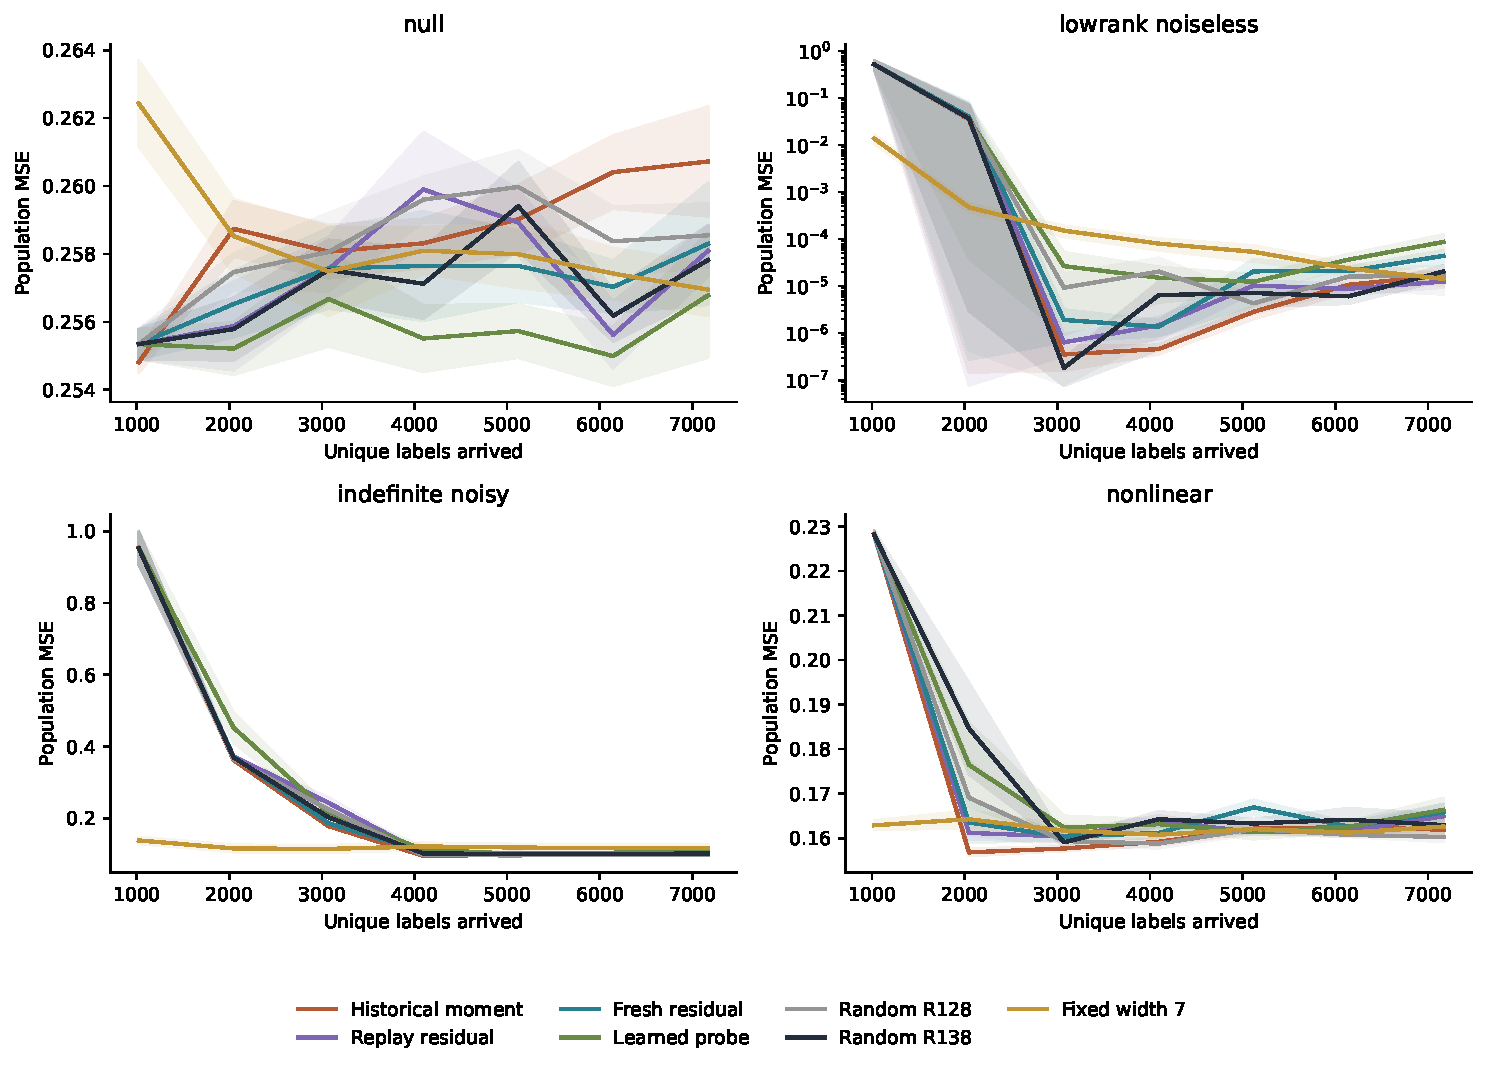
\includegraphics[width=\linewidth]{quadratic_trajectories.pdf}
\caption{Complete trained histories from saved outcomes. Bands are one
standard error across independent runs. All growing arms have the same
scheduled widths; improvements here concern direction and fitting mechanisms.
The rank-two panel uses a logarithmic risk axis.}
\end{figure}

\subsection{Same-checkpoint directions and finite-time refitting}
Lifetime histories diverge, so their final comparison cannot diagnose the
quality of identical candidate sets. We therefore froze a separate,
evaluator-only diagnostic. At every pre-growth checkpoint of the random-138
trajectory, all five direction mechanisms see the same current predictor,
optimizer state, retained rows and available data prefix. Each direction is
then followed by identical fitting work and minibatch randomness. Candidate
work is additional and logged, rather than claimed equal. Reconstructing a
historical moment from the archive explicitly charges all prefix rereads;
it does not purchase those labels again or retroactively give that storage
to the primary random learner. This adds 1,440 trained diagnostic branches.

For a quadratic task, the best possible output coefficient along a unit
vector $w$ yields gain $2\{w^\top(A-B)w\}^2$. This is computed from teacher
parameters only after training and never enters selection. Averaged first
within each seed over six checkpoints, historical directions exceed random
directions in this potential gain by $.08041\;[.04305,.11777]$ on rank-two
data and $.13116\;[.11530,.14702]$ on indefinite data. These are strong
initial direction differences.

After identical fully trainable refitting, the corresponding
historical-minus-random risk differences are
$2.713\times10^{-5}$, with interval $[-1.111,6.536]\times10^{-5}$, and
$-.002687\;[-.006656,.001282]$, respectively.
Neither interval resolves a refitted advantage. Better direction alignment
therefore does not by itself establish better learned models at the available
training budget. This directly limits the proposed mechanism, rather than
hiding a negative result behind a successful population direction formula.
The trained hidden vectors may move substantially; this diagnostic does not
claim that every source of erasure has been isolated.

\begin{figure}[tb]
\centering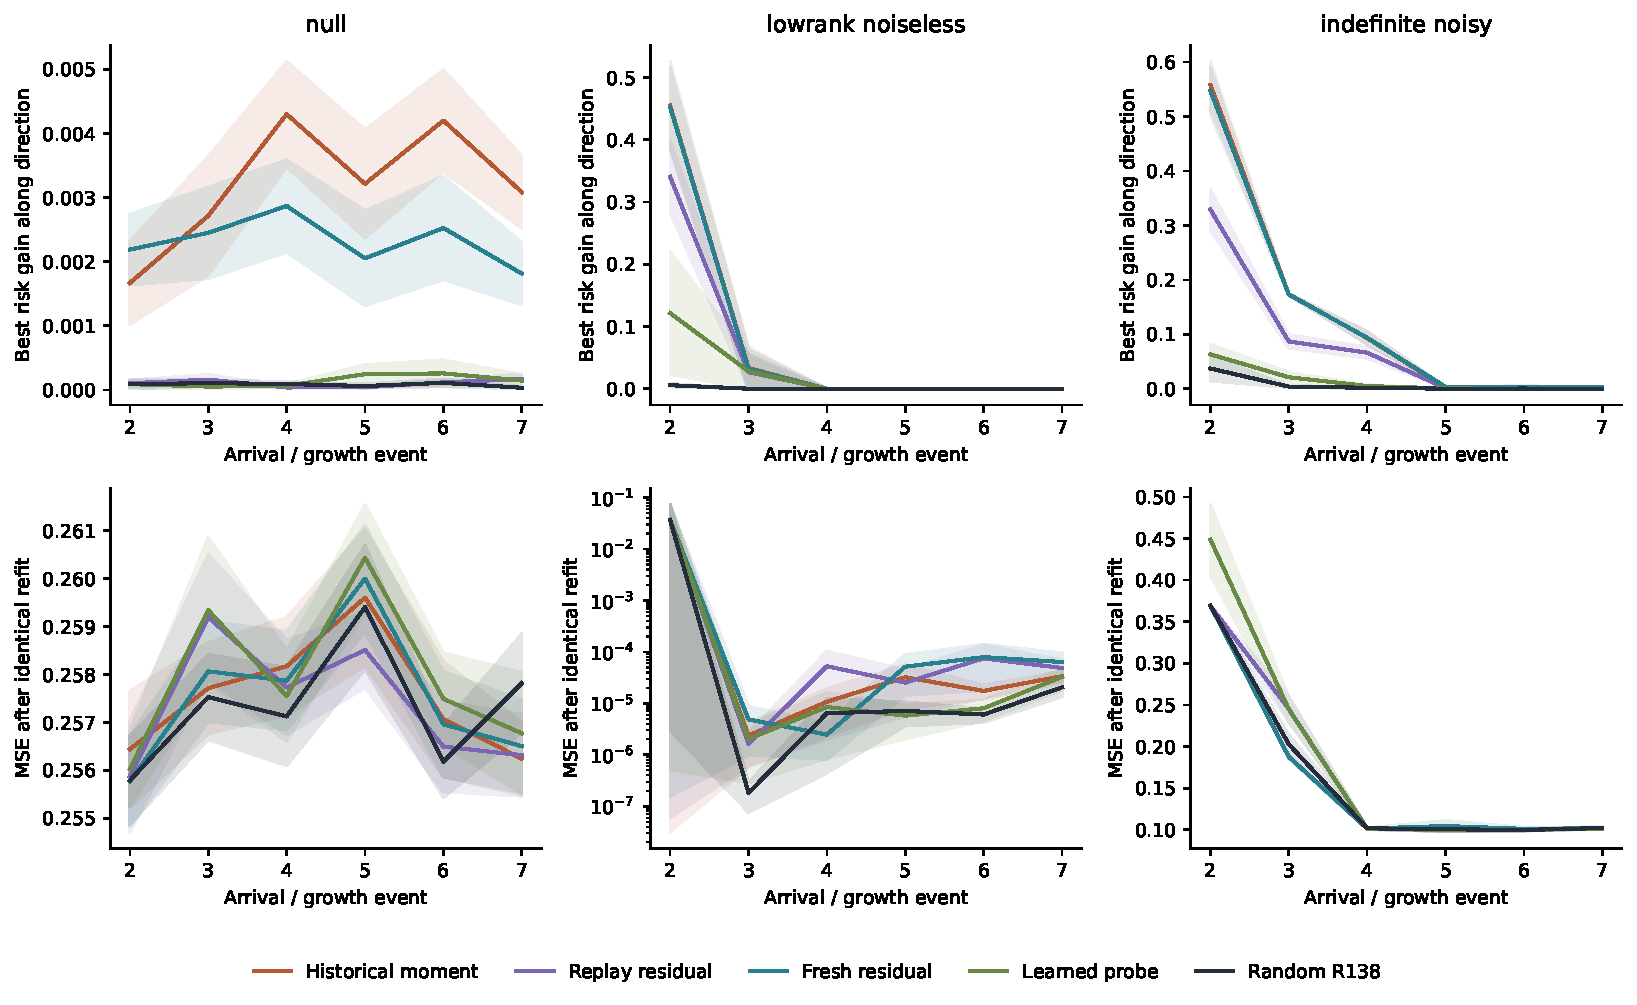
\includegraphics[width=\linewidth]{quadratic_checkpoint.pdf}
\caption{Same-checkpoint diagnostics. Top: evaluator-only best gain along
the supplied-to-refitting, data-discovered direction. Bottom: actual risk after
identical nonlinear refitting. These are different objects, and the large
initial direction gap need not remain a final learning advantage.}
\end{figure}

\subsection{Memory, computation and scientific limits}
Every primary arm spends approximately fourteen million arithmetic-proxy
units over its lifetime. Raw label accesses for fitting, proposals and moments
are saved by sample ID. Historical retention uses
$128(12+2)+144=1936$ eight-byte-word equivalents, including example labels and
identities; random 138 uses 1932. At final width seven, both additionally use
276 model/Adam words and six controller-state words. This comparison is nearly
matched in persistent algorithmic storage, not peak process memory. Current
blocks, duplicated fitting pools, candidate matrices, hidden optimizer state
and branch workspaces are separately reported. Python, BLAS/eigensolver
internals and evaluator/archive storage are excluded from the array ledger.

Numerical differentiation checks the model gradient to maximum absolute
error $3.52\times10^{-10}$ and a zero-output birth preserves predictions to
$3.47\times10^{-17}$. Raw archives contain observations, teacher/evaluator
information in separate fields, all parameters and optimizer snapshots,
source/configuration hashes and resource logs. Full result reconstruction
and external novelty review are separate from these implementation checks.
The main experiment neither establishes a new theorem nor a general neural
advantage. Its contribution to the investigation is a reproducible attempt
to learn structural directions, a failed attribution control, and direct
separation of population opportunity from finite-sample nonlinear learning.

\IfFileExists{adaptive_experiments.tex}{\section{A separate attempt at adaptive width}
\label{sec:adaptive-extension}

The controlled-direction study fixes width growth. To make a serious attempt
at actual structural adaptation, we separately implemented and froze a
fresh-seed extension that can grow, continue fitting, or hold. This extension
was designed after the main study and is exploratory; its outcomes do not
retroactively confirm a preselected main-study algorithmic claim.

\subsection{A deployable but heuristic controller}
The task laws, model, seven 1,024-label arrivals, arithmetic budget and optimizer
remain as above. Each arm retains 138 examples. Split each incoming block into
768 fitting/proposal labels and 256 validation labels. All candidate parameters
are finalized before the current validation labels are inspected. After the
action is committed, release the entire block into the reservoir, so completed
validation labels can support future fitting. Warmup on the initial 768 labels
is ungated. Future arrivals remain inaccessible.

Five arms compare fresh-residual growth, random growth, fixed width two with
validation, fixed width seven with validation, and fixed width seven without
validation. Growing learners begin at width one and can reach seven. At each
later opportunity, fit both a continuation and a zero-output-unit growth branch
from cloned incumbent optimizer states, splitting the remaining event budget
equally after charging proposals and validation predictions. Fixed arms spend
their remaining budget on continuation. Every rejected branch is charged.

For a candidate adding $r\in\{0,1\}$ units, let $\bar D$ and
$\widehat{\mathrm{se}}(D)$ be the mean and sample standard error of old-minus-new
squared losses on the 256 validation points. Qualify it when
\[
 \bar D>2\widehat{\mathrm{se}}(D)+.002+.001r.
\]
Install the qualifying candidate with largest mean gain minus $.002+.001r$,
or hold the exact incumbent if neither qualifies. This familiar holdout
pattern and the standard-error heuristic are not novel. Unbounded losses,
finite samples and unadjusted selection mean that we claim no population
safety guarantee. A rejection does not certify that the current representation
is adequate. This is deliberately separated from the earlier project's valid
bounded-loss audit theorem.

The protocol and source were frozen at 05:43:47 UTC on 20 September 2026,
before seeds 840000--840011. The 48 new paired configurations contain 240
complete trajectories and 1,680 events; all completed in 13.38 seconds on two
CPU workers. Source hashes, validation statistics, rejected branch parameters,
optimizer states, retained sample identities and all data access counts are
saved. A preflight perturbation of current validation labels leaves current
branch parameters unchanged and leaves earlier committed histories unchanged.
Descriptive intervals again use the twelve independent seeds, without a
multiple-comparison correction.

\subsection{Actual adaptive outcomes and retained failures}
\begin{table}[tb]
\centering\scriptsize
\begin{tabular}{lrrrr}
\toprule
Method & Null & Rank two & Indefinite & Nonlinear \\
\midrule
Fresh residual growth & 0.25366 (1.08) & 0.00014 (2.00) & 0.10033 (4.08) & 0.16204 (2.00) \\
Random growth & 0.25501 (1.17) & 0.00018 (2.08) & 0.10499 (4.17) & 0.16220 (2.00) \\
Fixed 2 gated & 0.25763 (2.00) & 0.07105 (2.00) & 0.52321 (2.00) & 0.18419 (2.00) \\
Fixed 7 gated & 0.26259 (7.00) & 0.00052 (7.00) & 0.10260 (7.00) & 0.16316 (7.00) \\
Fixed 7 ungated & 0.26506 (7.00) & 0.00002 (7.00) & 0.10175 (7.00) & 0.17007 (7.00) \\
\bottomrule
\end{tabular}

\caption{Separate adaptive extension: mean final MSE, followed by mean
committed width in parentheses. All results use new seeds; they are not paired
with the main study's seeds. Full marginal and paired intervals are saved.}
\label{tab:adaptive-results}
\end{table}

Fresh-residual growth learns mean final widths $1.08$, $2.00$, $4.08$ and
$2.00$ on null, rank-two, indefinite and nonlinear tasks. The respective
accepted additions across twelve runs are $1$, $12$, $37$ and $12$.
On the indefinite task, the method therefore makes repeated learned changes
within one lifetime, rather than restarting from a specially chosen point.
Random growth reaches widths $1.17$, $2.08$, $4.17$ and $2.00$, with
$2$, $13$, $38$ and $12$ accepted additions. All intermediate holds and
continuations are retained in the raw trajectories.

The fresh-minus-random final-risk difference on the indefinite task is
$-.004664$, with interval $[-.008976,-.000352]$. This favorable descriptive result is
limited to one task among several comparisons. Their differences on null,
rank-two and nonlinear tasks have intervals containing zero. In particular,
information-guided proposal learning has not earned a general claim to
superiority over random structural additions.

The wide fixed baselines limit the adaptive claim further. On indefinite
data, fresh-minus-fixed-seven gated is
$-.002269\;[-.005805,.001266]$ and fresh-minus-fixed-seven ungated is
$-.001418\;[-.006792,.003955]$: no resolved final-risk advantage, though
adaptation retains fewer units. On rank-two data the ungated fixed-seven
learner instead reaches mean error $2.15\times10^{-5}$ versus
$1.44\times10^{-4}$ for fresh growth, with paired adaptive-minus-fixed
interval $[.00000771,.00023663]$. Thus conservative commitments can stop
useful further fitting. The fixed-two gated arm is especially variable or
underfits; it is not used as the sole comparator.

Null outcomes distinguish restraint from learning adequacy. Fresh growth
holds at 67 of the 72 post-warmup opportunities and usually remains at width
one, but its mean risk $.253656$ still exceeds the Bayes risk $.25$.
Its rare accepted addition is not evidence that a true structural signal
exists. Good rejection behavior alone does not remove warmup or optimization
error. The nonlinear task similarly remains constrained by the chosen model
family, even when the controller stops adding units.

No accepted fresh-growth or random-growth step increased the evaluator risk
in these runs, but this observation is not a coverage guarantee. The same
heuristic did accept one evaluator-risk increase in the fixed-two rank-two
runs and one in its nonlinear runs; the latter evaluator is Monte Carlo.
All are retained. Ungated fixed-seven training has 33, 8, 28 and 36
risk-increasing steps across the four tasks. These numbers describe sampled
optimization histories and do not establish the statistical validity of the
heuristic gate.

\begin{figure}[tb]
\centering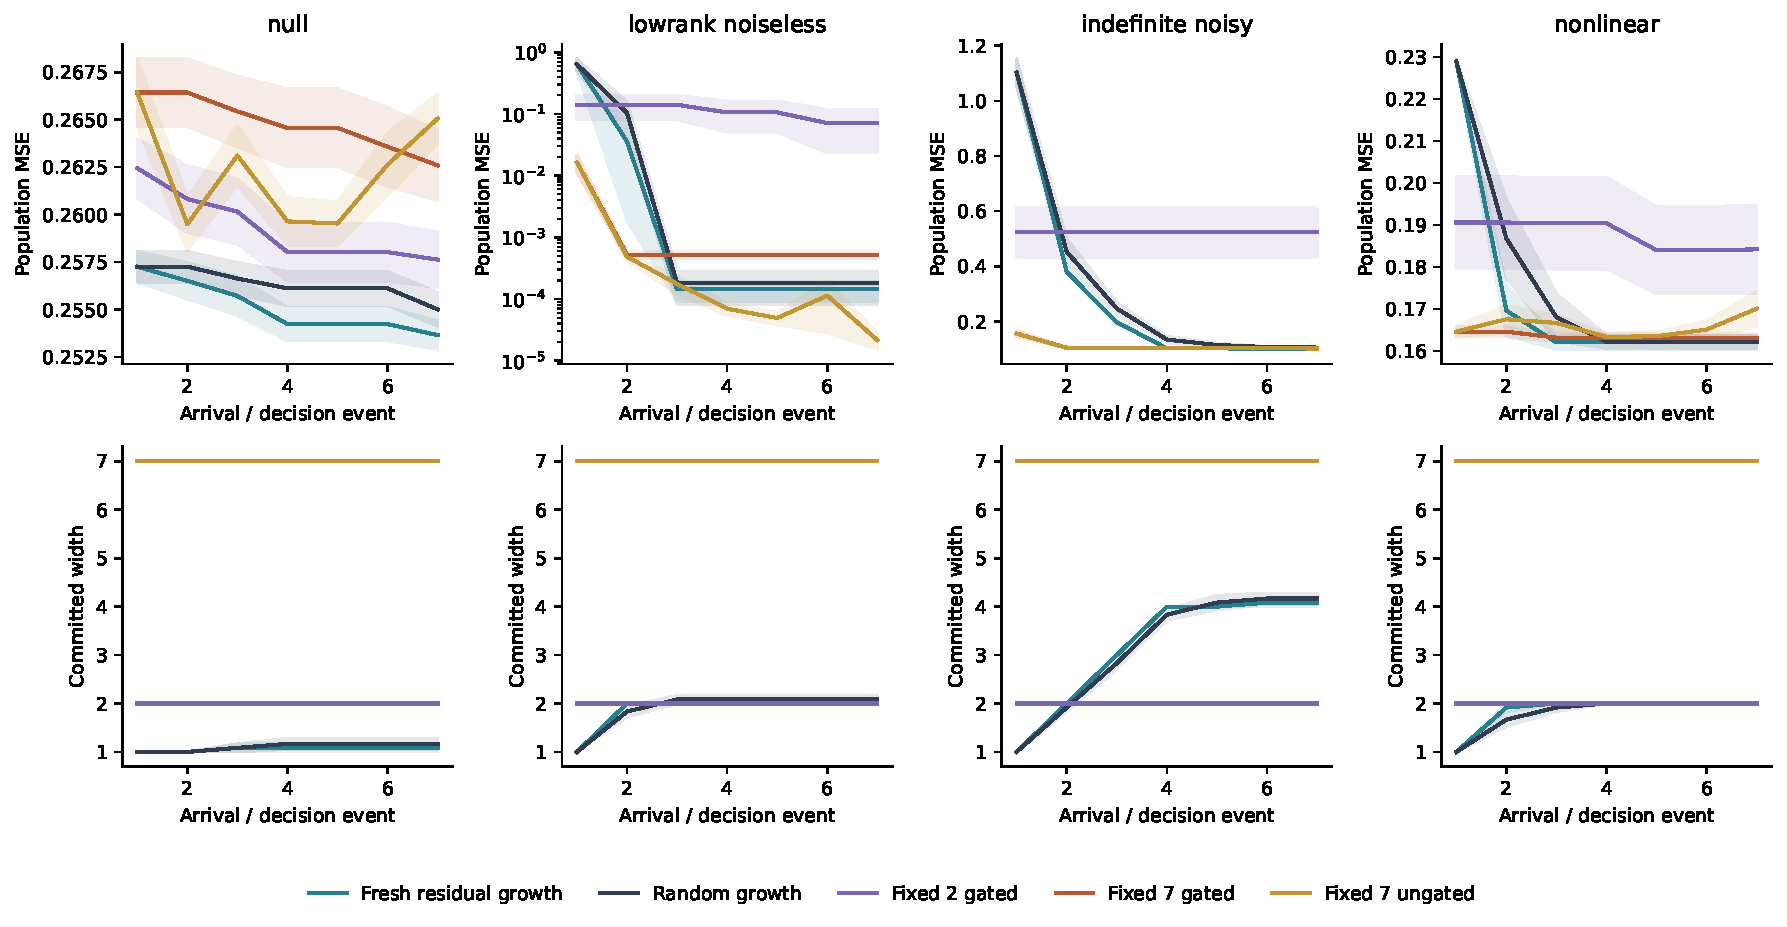
\includegraphics[width=\linewidth]{adaptive_trajectories.pdf}
\caption{Separate fresh-seed adaptive histories. The upper row shows risk;
the lower row shows actually committed widths. Bands are one standard error.
The opportunity schedule is precommitted, while directions and accepted widths
are chosen from observed data.}
\end{figure}

\subsection{Cost and interpretation}
All arms consume approximately fourteen million charged arithmetic-proxy
units. For fresh growth, rejected branches alone consume mean totals of
10.62, 9.83, 7.79 and 9.83 million across the four tasks. These costs are not
hidden behind the smaller deployed width. Fixed wide learners have greater
persistent optimizer storage from the start, while adaptive candidates require
additional simultaneous branch storage; the separate ledgers expose both.
No equal-width or equal-proxy statement is promoted to equal physical memory
or equal wall-clock computation.

This extension realizes data-dependent architecture selection with learned
hidden vectors, ordinary starts, label release and strong online controls.
It does not establish a novel growth principle, a valid universal gate,
optimal rank discovery, or publication readiness. Its favorable indefinite
comparison, negative fixed-capacity comparison, false-risk-decrease episodes,
and substantial rejected computation are all part of the result.
}{}
\section{A targeted response to the minibatch confound}
\label{sec:fullbatch}

We did not stop at documenting the different tail batches in the original
replay comparison. A separately frozen follow-up clones the primary runner
and changes the fitting batch assembly: carry the end of a shuffled pool
into a new independent permutation until a full 128-example batch is formed.
Only the final arithmetic-budget remainder can form a smaller batch. All
models, task laws, proposal rules, optimizer settings, data arrivals and
resource charges remain unchanged. The original source and outcomes are
preserved. This is a targeted post-hoc investigation, not a retroactive
replacement of the main experiment.

Before running seeds 850000--850011, we froze the derived source, four-arm
configuration and protocol at 05:49:36 UTC on 20 September 2026. The arms are
historical moments with replay 128, random growth with replay 128 and 138,
and fixed width seven with replay 138. We omit the separate paired-branch
diagnostic here, as specified before execution. The 48 new configurations
produce 192 complete trajectories and 1,344 events in 9.76 seconds. Every
random-128 and random-138 run now has exactly 975 optimizer updates and
124,285 fitting-example accesses. Their example counts, update counts and
minibatch-size sequences are thus matched, while their retained samples can
still differ. Historical moments spend candidate work and use 892 updates;
fixed width seven uses 392 updates, reflecting its larger per-example cost.

\begin{table}[tb]
\centering\small
\begin{tabular}{lrrrr}
\toprule
Method & Null & Rank two & Indefinite & Nonlinear \\
\midrule
Historical moment & 0.260777 & 0.000022 & 0.096205 & 0.162987 \\
Random R128 & 0.259258 & 0.000047 & 0.098319 & 0.161161 \\
Random R138 & 0.259687 & 0.000012 & 0.096821 & 0.163098 \\
Fixed width 7 & 0.259182 & 0.000021 & 0.104035 & 0.159968 \\
\bottomrule
\end{tabular}

\caption{New-seed, full-minibatch follow-up. These are separate observations,
not overwritten entries in Table~\ref{tab:quadratic-results}. All means are
final population MSE, with the same nonlinear Monte Carlo evaluation rule.}
\label{tab:fullbatch}
\end{table}

The original adverse indefinite-task comparison between replay sizes does
not persist. Random-128 minus random-138 is now $+.001498$, with interval
$[-.001121,.004117]$, compared with the original negative estimate
$-.005038$ and interval $[-.007834,-.002243]$. Historical moments minus
random-138 is $-.000616$, with interval $[-.001736,.000504]$; historical
moments minus random-128 is $-.002114$, with interval
$[-.004453,.000226]$. Both intervals include zero.
Thus a general learning benefit from retaining the target moment is not
established by this follow-up. On the other tasks, all targeted historical
and replay-size paired intervals likewise include zero. That statement is a
failure to resolve effects, not an equivalence proof.

The changed update schedule is mechanically verified, and the new empirical
comparisons fail to support the original strong attribution. Because the
follow-up uses new seeds, the difference between old and new point estimates
is not itself a paired causal estimate of the minibatch correction. The
correct conclusion is narrower: the original comparison was confounded,
and the proposed moment advantage has not survived the present control with
matched minibatch schedules. A stronger assessment would randomize or pair
both batching schedules on an additional untouched seed set, ideally with
an optimizer-budget definition chosen in advance.

\begin{figure}[tb]
\centering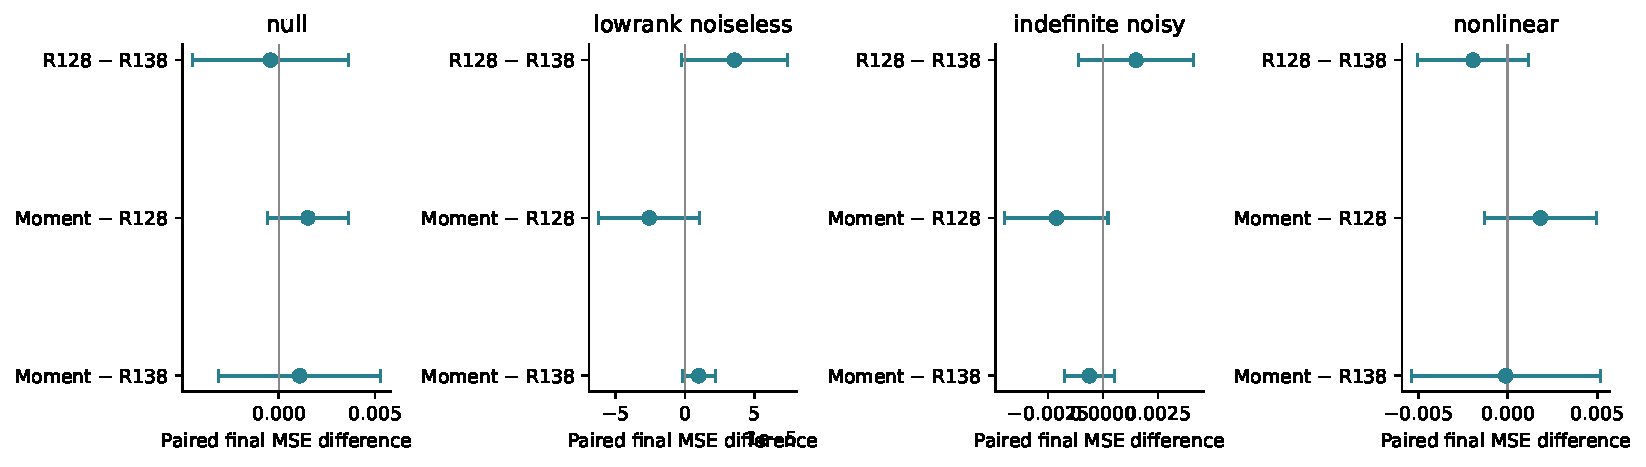
\includegraphics[width=\linewidth]{fullbatch_followup.pdf}
\caption{Targeted paired risk differences after removing epoch-tail changes
in update count. Bars are descriptive 95\% Student-$t$ intervals over twelve
independent new seeds; no multiplicity adjustment is made. None of these
intervals establishes a resolved final-risk advantage.}
\end{figure}

Across the primary, adaptive and targeted studies there are 768 complete
confirmation/follow-up trajectories, plus 1,440 same-checkpoint trained
branches. This volume is evidence of implementation and investigation,
not a substitute for a surviving theorem-level novelty claim or a robust
empirical improvement. The unsuccessful attribution remains part of the
research result.


\section{What the investigation establishes and leaves unresolved}
\label{sec:limits}
The distinction between a population inverse and empirical residual
subtraction is exact and matters even without label noise. A stored matrix
can contain genuinely data-discovered directions while repeated processing
of it adds no new evidence. Updating that matrix by subtracting current
predictions at the sample level is a different operation, and fresh inputs
permit a clean conditional calculation. These are useful constraints on the
original information-driven learning idea: the relevant information must
support the \emph{current} optimization operator, not only its expectation
at a fixed independent model.

The current results do not finish the intended contribution. They provide
no finite-precision lower bound for all learners, no optimal unknown-rank
sample-and-runtime result, no global guarantee for hidden-weight Adam, and
no evidence that neuron-local information measures beat strong existing
search procedures. The Gaussian model is a controlled setting with an exact
population inverse; unknown or non-Gaussian covariate laws require additional
estimation. The matrix correction theorem is not the trained factor-Adam
algorithm, and the main direction experiment has scheduled widths. A
heuristic gate does not acquire a false-acceptance theorem by sharing a
fresh-block data schedule.

Storage is accounted for through named arrays and access logs; physical
peak memory and floating-point roundoff are not bounded theoretically.
Inference width, persistent learner state, working arrays, saved scientific
records, and evaluator storage are separate resources. Near-matched replay
storage does not imply matched total memory, exact FLOPs, or hardware time.
Uncertainty intervals use independent seeds, not time points or branch
proposals. They are descriptive and not multiplicity-adjusted. The finite
synthetic task set supports no universal performance claim.

A substantive next theorem would need a consequence beyond existing
optimal recovery, coreset approximation, spectral thresholding, and
stochastic low-rank optimization. One precise target is noisy,
unknown-rank online discovery with an explicit approximation oracle bound
and an accountable advantage under a declared memory--work frontier. A
proof must not silently import an ordinary RIP that the measurements lack,
and an empirical improvement must survive competent fixed-rank and
matrix-free alternatives. The present evidence does not establish that
such an advantage exists. If these comparisons subsume the next candidate,
it should be rejected rather than renamed.

\section{Reproduction and evidence integrity}
The companion workspace preserves source versions, raw observations,
per-run parameters, fitting/proposal accesses, all figure scripts, and
independent reports. \texttt{README.md} gives a minimal verification command
and complete re-execution instructions into new destinations. Each
confirmatory protocol was frozen before its own confirmation seeds ran.
Development fixes, source-hash differences, accounting corrections and
post-hoc analytic diagnostics are recorded explicitly. Prior artifacts are
checked against the baseline manifest. No earlier result is overwritten,
and no external publication, submission, paid compute or private-data
upload was performed.

\appendix
\section{A literal-assumption caveat in a current spectral theorem}
\label{app:source}

We checked Defilippis et al.~\cite{defilippis}, arXiv:2602.05846v1,
on 20 September 2026 UTC: Definitions 2.1--2.7 and 3.3,
Assumptions 2.3--3.4, Theorem 3.6, and Appendix A.2. The current record
listed only v1, dated 5 February 2026. The spectral estimator uses
\[
 M=\sum_{i=1}^n\mathcal T(Y_i)X_iX_i^\top,
 \qquad X_i\sim N(0,I_d/d),
\]
with eigenvalue-gap selection and eigenvector norm $\sqrt d$.
The preprocessing conditions are boundedness, positive essential
supremum, and a nonzero value with positive probability. We test only
the literal universal preprocessing scope of the rate claim, not other
results or a qualified theorem. This is not our main originality claim.

\begin{proposition}[Constant preprocessing fails the literal universal claim]
\label{prop:source-constant-preprocessing}
Take orthogonal target directions $w_k^*$ with $\|w_k^*\|_2^2=d$,
$1\leq k\leq m_*\leq d$, and normalized weights
\[
 a_k=\frac{k^{-\gamma}}{\left(\sum_{j=1}^{m_*}j^{-2\gamma}\right)^{1/2}},
 \qquad \gamma>\frac12.
\]
Let $g_k(z)=(z^2-1)/\sqrt2$ and
\[
 Y=\sum_{k=1}^{m_*}a_kg_k(\langle w_k^*,X\rangle)
          +\sqrt\Delta\,\xi,
 \qquad \Delta>0,\quad \xi\sim N(0,1),
\]
with $X$ and $\xi$ independent. Choose $\mathcal T(y)=1$.
For $n\geq d\geq2$, select any number $r\leq m_*$ of the ordered
eigenvectors of $M$ by a rule depending only on its eigenvalues,
normalize them to $\sqrt d$, and pad the remaining output rows by zero.
The resulting weighted matrix reconstruction error satisfies
\begin{equation}
 \sum_{k=1}^{m_*}\frac{a_k^2}{d^2}
 \mathbb E\left[
 \|\widehat w_k\widehat w_k^\top-w_k^*w_k^{*\top}\|_F^2
 \right]\geq1.
 \label{eq:source-lower-error}
\end{equation}
The expectation is over the input sample; the assertion also holds for
random orthogonal teachers independent of those inputs.
\end{proposition}
\begin{proof}
The links are even polynomials with
$\mathbb E[g_k(Z)^2]=1$ and
$\mathbb E[g_k''(Z)]=\sqrt2$ for $Z\sim N(0,1)$.
They have a uniform polynomial envelope and satisfy the displayed
nondegeneracy conditions on the target. The weights are strictly
decreasing, have sum of squares one, and satisfy the required power-law
scaling with constants independent of $m_*$, because $\gamma>1/2$.
The preprocessing is bounded, is never zero, and has the specified
positive essential supremum:
\[
 \inf\{c:\mathbb P(\mathcal T(Y)<c)=1\}
 =\inf(1,\infty)=1.
\]
Thus it meets the literal preprocessing conditions.

With this choice, $M=\sum_iX_iX_i^\top$ depends only on isotropic
Gaussian inputs. It is a rotationally invariant Wishart matrix,
independent of any information about target directions in the labels.
For $n\geq d$ its eigenvalues are distinct almost surely. Conditional on
the ordered eigenvalues, every normalized rank-one eigenprojector is
uniformly oriented. In particular, for an eigenvector $v$ normalized by
$\|v\|_2^2=d$,
\[
 \mathbb E[vv^\top\mid\operatorname{spec}(M)]=I_d,
 \qquad
 \mathbb E[(v^\top w_k^*)^2\mid\operatorname{spec}(M)]=d.
\]
These statements concern projectors and hence do not depend on how the
sign of an eigenvector is chosen. Selection of $r$ through eigenvalues
also leaves them unchanged. Consequently every selected row has
conditional normalized error
\[
 \frac{\mathbb E[\|vv^\top-w_k^*w_k^{*\top}\|_F^2
              \mid\operatorname{spec}(M)]}{d^2}
 =\frac{d^2+d^2-2d}{d^2}=2-\frac2d.
\]
A zero-padded row has normalized error one. If $p_k$ is the probability
that row $k$ is selected, the left side of
\eqref{eq:source-lower-error} is therefore
\[
 \sum_{k=1}^{m_*}a_k^2
       \left\{p_k\left(2-\frac2d\right)+(1-p_k)\right\}
 =1+\left(1-\frac2d\right)\sum_{k=1}^{m_*}a_k^2p_k\geq1.
\]
Conditioning first on a random teacher gives the same conclusion when
the teacher is independent of the inputs.
\end{proof}

The literal rate assertion combines Theorem 3.6 with the displayed
large-sample regime $\alpha=n/d\gg m_*^{2\gamma}$, in which the claimed
weighted optimal rate is of order $m_*/\alpha$. That rate can tend to
zero, whereas \eqref{eq:source-lower-error} cannot. For example, in the
subsequent large-$\alpha,m_*$ comparison, taking
$\alpha=m_*^{2\gamma+1}$ gives $m_*/\alpha=m_*^{-2\gamma}$.
The disagreement persists after the proportional high-dimensional limit,
since the lower bound holds at every finite $d\geq\max(m_*,2)$.
Likewise, normalized squared overlap of any selected row with a fixed
target direction is $1/d$, so no fixed finite $\alpha$ yields weak
recovery from this input-only estimator.

The source proof's transition from its equations (66) to (70) has a
leading coefficient containing
$\int\mathcal T(y)\mathsf Z'(y)\,\mathrm dy$.
For the constant preprocessing this is zero: $\mathsf Z$ is a Gaussian
convolution density, tends to zero at both ends, and has an integrable
derivative, so its derivative integrates to zero. Boundedness and
nonzero preprocessing do not imply a nonzero appropriately signed
coupling to the target. An added coupling condition, or a specified
valid preprocessing family, would be a substantive qualification to
check in a corrected theorem. This observation does not supply a new
learning mechanism for our project.

\section{Exact approximation floor for the nonlinear stress task}
\label{app:nonlinear}
This analytic diagnostic was developed after the primary protocol was
frozen. It does not change training, tuning, or the original Monte Carlo
endpoint. Let $Z_1,Z_2,Z_3$ be independent standard normal coordinates after
an orthogonal rotation, and let
\[
 f_*(Z)=.8\tanh(1.5Z_1)\tanh(1.5Z_2)+.4\sin Z_3.
\]
Define
\[
 a=\mathbb E[Z\tanh(1.5Z)],\quad
 b=\mathbb E[\tanh^2(1.5Z)],\quad c=.8a^2.
\]
\begin{proposition}[A width-independent approximation obstruction]
The orthogonal projection of $f_*$ onto the class of all centered quadratic
forms plus constants is $cZ_1Z_2$. If $u_1,u_2$ are the corresponding
orthonormal directions and
$A_0=\frac c2(u_1u_2^\top+u_2u_1^\top)$, then every quadratic network,
of arbitrary width, with matrix $B$ and intercept $c_0$ satisfies
\[
 \mathbb E[(f_*(X)-q_B(X)-c_0)^2]
 =F_0+2\|B-A_0\|_F^2+c_0^2,
\]
where
\[
 F_0=.64b^2+.08(1-e^{-2})-.64a^4.
\]
The best predictor is realizable by two signed quadratic neurons.
\end{proposition}
\begin{proof}
A centered quadratic form is a linear combination of $Z_i^2-1$ and
$Z_iZ_j$, $i<j$. Independence and oddness imply that $f_*$ has zero
mean and zero inner product with every diagonal term. The product of two
odd hyperbolic tangents has zero correlation with every cross term except
$Z_1Z_2$; for that term the correlation is $.8a^2=c$, while
$\mathbb E[Z_1^2Z_2^2]=1$. The sine term is odd under $Z\mapsto-Z$ and
is orthogonal to every quadratic form and to constants. These facts identify
the projection.

The two components of $f_*$ are orthogonal, with squared norms $.64b^2$
and $.16\mathbb E\sin^2 Z=.08(1-e^{-2})$, respectively; the latter follows
from $\sin^2 z=(1-\cos2z)/2$ and the Gaussian characteristic function.
Subtracting the projection's squared norm $c^2$ yields $F_0$. The
Pythagorean identity and Theorem~\ref{thm:quadratic-geometry} give the risk
formula. Finally, $A_0$ has eigenvectors $(u_1+u_2)/\sqrt2$ and
$(u_1-u_2)/\sqrt2$, eigenvalues $c/2$ and $-c/2$, so two signed neurons
suffice.
\end{proof}
One-dimensional numerical quadrature gives
$a\approx.689027429$, $b\approx.540648381$, $c\approx.379807038$ and
$F_0\approx.111992221$. The added observation-noise variance $.04$ makes
the best total squared risk approximately $.151992221$. These values are
numerical evaluations of the displayed expectations, not additional
statistical estimates. The script \texttt{code/nonlinear\_projection.py}
reproduces the quadrature and evaluates saved final parameters using this
identity. Those post-hoc analytic evaluations are stored separately; all
original Monte Carlo primary outcomes remain unchanged. The sine component alone contributes an irreducible
$.069173177$ for this architecture. More width cannot remove this
misspecification. Information-guided adaptation would need to change the
function family, not merely discover additional quadratic directions.

\bibliographystyle{plainnat}
\bibliography{references}
\end{document}
